%!TEX root = main.tex
\section{Evaluation}
\label{sec:evaluation}
\subsection{Experimental setup}
\textbf{Server.}
We conducted the experiments on the server which is
equipped with 8 NVIDIA Tesla A100 GPUs, each with 40 GB of memory, PCIe 4.0 $\times$16,
an AMD EPYC 7402 2.8 GHz 24-core processor, and 504 GB of memory.
The server is installed with CentOS 7, the CUDA Toolkit 11.2 and cuDNN 8.4.1,
with PyTorch version 1.11, and Huggingface Transformers~\cite{wolf2020transformers} version 4.27.2. The NCCL library version is 2.10.3.

\textbf{Workloads.}
% \subsubsection{Workloads}
We conduct the evaluation on four state-of-the-art deep learning models, including:
BERT~\cite{devlinBERTPretrainingDeep2019}, GPT-2~\cite{radfordLanguageModelsAre2019}, T5 (Text-to-Text Transfer Transformer)~\cite{raffelExploringLimitsTransfer2020}, and AmoebaNet~\cite{realRegularizedEvolutionImage2019}.
BERT is proposed by Google AI Language which contains 1024 hidden layers and approximately 340 million parameters.
GPT-2 is a famous pre-trained model proposed by OpenAI,
which has achieved remarkable success in various NLP tasks.
We uses the large version in the evaluation which contains about 770 million parameters.
T5 is a sequence-to-sequence model proposed by Google.
We uses its large version which contains about 780 million parameters.
AmoebaNet is a neural network that is automatically generated by the Neural Architecture Search (NAS) algorithm,
which contains about 28 million parameters
% evolutionary strategy based on the genetic algorithm in neural network architecture search,
BERT and GPT-2 are both trained with the WikiText-103~\cite{merityPointerSentinelMixture2017} dataset and T5 uses the WMT-16~\cite{bojarFindings2016Conference2016} dataset.
These three models are trained with \emph{Adam} optimizer.
The AmoebaNet model is trained with the ImageNet~\cite{dengImagenetLargeScaleHierarchical2009} dataset and the stochastic gradient descent (SGD) optimizer.
Two configurations with pipeline stage numbers of 4 and 8 are tested.

\textbf{Baselines.}
We have set up four baselines to evaluate the memory efficiency and training performance, which are listed below.
% The memory efficiency is represented by the maximum trainable batch size
% Since there is no clear interval between the computation of two batches in asynchronous training
% as in synchronous training, it is not possible to compare the batch sizes equally between synchronous
% and asynchronous training. Therefore, this chapter compares the batch sizes separately when comparing them,
% and their detailed introductions are as follows.
\begin{itemize}
  \item ZeRO~\cite{rajbhandariZeROMemoryOptimizations2020}: It is developed by Microsoft to eliminate redundant storage related to parameters
  across GPUs in data parallel training.
  We select the optimization levels two and three, namely ZeRO-2 and ZeRO-3, in this evaluation.
  \item GPipe~\cite{huangGpipeEfficientTraining2019}: Since the original GPipe is implemented based on the Lingvo~\cite{shen2019lingvo} framework,
  we use torchgpipe~\cite{kimTorchgpipeOntheflyPipeline2020} instead for evaluation which is an re-implementation of GPipe on PyTorch.
  \item PipeDream~\cite{narayananPipeDreamGeneralizedPipeline2019}: It firstly profiles the model in runtime and then uses dynamic programming
  to make the longest computation time among all stages as small as possible.
  % It is an asynchronous pipeline parallel method proposed by Narayanan et al,
  % which adopts a 1F1B computation scheduling method in each stage to eliminate pipeline bubbles.
  % PipeDream first measures and analyzes the model to obtain the execution characteristics of the model,
  % and then uses dynamic programming to make the longest computation time in all divided stages
  % after division as small as possible. The open-source implementation of PipeDream is based on PyTorch.
  \item vPipe~\cite{zhaoVPipeVirtualizedAcceleration2022}: It is implemented based on the runtime of PipeDream.
  However, its partition algorithm is not open-sourced yet.
  By that, we have implemented the algorithm according to the description in the corresponding paper of vPipe.
  % It is a pipeline division method that comprehensively considers model division,
  % memory exchange, and re-computation, proposed by Zhao et al.
  % It adopts an iterative algorithm to dynamically find a balance between model division and memory optimization.
  % It is implemented based on the runtime system of PipeDream.
  % Since the division algorithm of vPipe is not open-sourced,
  % this chapter implements the corresponding model division algorithm in PipeDream
  % based on the algorithm description in the corresponding paper of vPipe.
  % In this section, vPipe-S is used to represent the synchronous pipeline parallel model of vPipe,
  % and vPipe-AS is used to represent the asynchronous pipeline of vPipe.
\end{itemize}

\subsection{Memory Using Efficiency}
In this section, we evaluate the maximum trainable batch size of each method
to reflect the GPU memory usage efficiency.
We use the micro batch size to compare in asynchronous pipeline parallel training
since it is not like synchronous training which has a
clear interval between the computation of two batches.
% Since there is no clear interval between the computation of two batches in asynchronous training
% as in synchronous training, it is not possible to compare the batch sizes equally between synchronous
% and asynchronous training. Therefore, we compares the batch sizes separately when comparing them,

% Since some methods use memory optimization techniques such as memory swapping and
% re-computation to increase the trainable batch size, such as GPipe and vPipe,
% and to compare the increase in batch size brought by different methods,
% we will compare methods without memory optimization with those that use memory optimization.

\subsubsection{Synchronous Pipeline Parallel Training}
We firstly perform the evaluation in the synchronous pipeline parallel training mode.
The number of micro-batches is equal to the pipeline stages in this experiment.
% First, a comparison of each method under the synchronous training model is made.
% In this mode, the batch size is equal to the micro-batch size multiplied by the number of splits.
% In this experiment, the number of splits is set to the number of pipeline stages.
The results are shown in Table~\ref{table:maxbs-sync},
and the synchronous training mode of vPipe and DawnPiper
are denoted as vPipe-S and DPiper-S, respectively.

It can be seen that ZeRO-2 and ZeRO-3 can achieve basically
the same maximum batch size on the four models,
and the maximum batch sizes of ZeRO-3 are even smaller on the T5 and AmoebaNet models.
This is because the extra memory space of memory optimization on model parameters of ZeRO-3
as the batch size increases,
the optimization of ZeRO-3 for the memory occupation of model parameters is no longer
sufficient to support a larger batch,
and it also requires additional memory buffers for communication.
For the results of GPipe and vPipe, it can be seen that the maximum batch sizes are basically
consistent with ZeRO on BERT, GPT-2, and T5.
% the maximum trainable batch size is basically consistent with the data parallel method optimized by ZeRO.
However, the batch sizes are much smaller than ZeRO on the AmoebaNet model.
This is because the Transformer-based models where the computation
and memory occupation of each layer are basically proportional,
making the division method of GPipe and vPipe,
which aims at balancing the computation time among stages,
also able to make the memory footprint of each stage basically balanced.
% However, on the AmoebaNet model, this batch size is much smaller than ZeRO,
% which is due to the Transformer-based models where the computation and memory occupation of each layer
% are basically proportional, making the division method of GPipe and vPipe-S, which aims at balancing
% the computation time between stages, also able to make the memory occupation between stages more balanced.
The situation is different on CNN models, where the computation
and memory occupation of layers are usually not proportional, that is,
a layer may have a long computation time but its memory usage may be very small,
such as the convolutional layer, which leads to a very uneven memory footprint
when trying to balance the computation time of each stage.
% under the condition of balanced computation time in each stage.
% AmoebaNet is a CNN model, where the computation and memory occupation of layers are not proportional, that is,
% a layer may have a long computation time but its memory occupation may be very small,
% such as the convolutional layer, which leads to a very uneven memory occupation under the condition
% of balanced computation time in each stage.
As a result, the maximum batch size that GPipe and vPipe can achieve
on the AmoebaNet model is 68\% and 46\% of ZeRO when the number of pipeline stages is 4.
This ratio becomes even smaller, only 58\% and 32\% as the number of pipeline stages increases to 8.
% Therefore, when the number of pipeline stages is 4,
% the maximum batch size that GPipe and vPipe-S can achieve on the AmoebaNet model is 68\% and 46\% of ZeRO, respectively.
% When the number of pipelines increases to 8, this ratio becomes even smaller, only 58\% and 32\%.
In the meantime, it is noted that GPipe can achieve a larger batch size compared to vPipe,
while the results are reversed after enabling memory optimization.
It is because the stage of the memory bottleneck becomes different when enabling memory optimization.
% because after enabling memory optimization,
% the stages that become the memory bottleneck in GPipe and vPipe-S are different.

DawnPiper achieves the largest batch size among all methods on the BERT, GPT-2, and T5.
Without memory optimization, it can increase the batch size by up to 1.2$\times$ and 1.55$\times$
compared to the second best method, vPipe, when the pipeline stages are 4 and 8, respectively.
% when there is no memory optimization.
% Without enabling memory optimization, it can increase the batch size by up to 1.2$\times$ and 1.55$\times$
% compared to the next best method, vPipe-S, when the pipeline stage is 4 and 8, respectively.
Note that the maximum batch sizes are consistent across all methods for GPT-2
due to its significant memory footprint during training.
Even a slight increase in batch size results in a notable increase in memory usage.
% the memory footprint during the training is significantly large.
Although DawnPiper can refine the pipeline partition space,
it cannot further increase the batch size.
% It should be noted that for the GPT-2 model, the maximum batch size is the same across all methods.
% This is because its model training memory occupation is very large, and due to its model structure characteristics,
% the memory occupation of each stage is also quite similar when evenly divided by computation.
% Although DawnPiper-S can refine the model division space,
% it cannot further increase the batch size.
For AmoebaNet, the maximum batch size of DawnPiper is slightly smaller than ZeRO,
since the data parallelism can perfectly divide the memory footprint of each GPU,
which is difficult to achieve in pipeline parallelism.
% because for smaller CNN models,
% data parallelism can perfectly divide memory occupation,
% which is difficult to achieve in pipeline parallelism.
Nonetheless, DawnPiper can increase by 1.29$\times$ and 1.91$\times$
compared to GPipe and vPipe when the pipeline stages is 4.
It can still outperforms GPipe and vPipe by up to 1.17$\times$ and 2.12$\times$
as the number of stages increases to 8.
% However, when the pipeline stage number is 4, DawnPiper-S can increase by 1.29$\times$ and 1.91$\times$
% compared to GPipe and vPipe-S, respectively.
% When it is increased to 8, it can also increase by 1.17$\times$ and 2.12$\times$, respectively.
DawnPiper still achieves the biggest batch size after the memory optimization is enabled.
Compared to the second best method, vPipe, the maximum batch size is increased
by an average of 1.33$\times$ and 1.29$\times$ when the pipeline stage is 4 and 8, respectively.
Additionally, it can be seen that the average batch size that
DawnPiper can achieve is increased by 1.84$\times$
as the number of pipeline stages is doubled,
indicating that DawnPiper shows a good memory scalability.
% When memory optimization is enabled, it can be seen that DawnPiper-S still achieves
% the largest batch size among all methods.
% On the 4 models, compared to the next best method, vPipe-S, the maximum batch size is increased
% by an average of 1.33$\times$ and 1.29$\times$ when the pipeline stage is 4 and 8, respectively.
% By comparing the maximum batch sizes that DawnPiper-S can achieve on the 4 models when the pipeline stages
% are 4 and 8, respectively, it can be seen that when the number of GPUs is doubled,
% the average batch size that DawnPiper-S can achieve is increased by 1.84$\times$,
% indicating that the method proposed in this study has very good memory scalability.

\begin{table}[htbp]
  \centering
  \caption{Maximum Batch Size in Synchronous Pipeline Parallelism}
    \begin{tabular}{m{2em}|m{2em}|ccccc}
    \toprule
    \#\ GPU & MO & Method & BERT & GPT-2 & T5 & AmoebaNet \\
    \midrule
    \multirow{8}{*}{4} & \multirow{5}{*}{None} & ZeRO-2 & 64    & 8     & 140   & 412 \\
          &       & ZeRO-3 & 64    & 8     & 132   & 404 \\
          &       & GPipe & 52    & 8     & 144   & 280 \\
          &       & vPipe-S & 60    & 8     & 144   & 188 \\
          &       & \textbf{DPiper-S} & \textbf{72} & \textbf{8} & \textbf{160} & \textbf{360} \\
\cmidrule{2-7}          & R & GPipe & 120   & 28    & 348   & 644 \\
\cmidrule{2-2}          & \multirow{2}{*}{S+R} & vPipe-S & 128   & 28    & 348   & 720 \\
          &       & \textbf{DPiper-S} & \textbf{160} & \textbf{32} & \textbf{424} & \textbf{1220} \\
    \midrule
    \multirow{8}{*}{8} & \multirow{5}{*}{None} & ZeRO-2 & 128   & 16    & 224   & 824 \\
          &       & ZeRO-3 & 128   & 16    & 208   & 808 \\
          &       & GPipe & 88    & 16    & 256   & 480 \\
          &       & vPipe-S & 88    & 16    & 256   & 264 \\
          &       & \textbf{DPiper-S} & \textbf{136} & \textbf{16} & \textbf{320} & \textbf{560} \\
\cmidrule{2-7}          & R & GPipe & 208   & 48    & 664   & 1384 \\
\cmidrule{2-2}          & \multirow{2}{*}{S+R} & vPipe-S & 208   & 56    & 664   & 1424 \\
          &       & \textbf{DPiper-S} & \textbf{280} & \textbf{60} & \textbf{800} & \textbf{2180} \\
    \bottomrule
    \end{tabular}%
  \label{table:maxbs-sync}%
\end{table}

% Table generated by Excel2LaTeX from sheet '工作簿2'
\begin{table}[htbp]
  \centering
  \caption{Maximum Batch Size in ASynchronous Pipeline Parallelism}
    \begin{tabular}{m{2em}|m{2em}|m{5em}cccc}
    \toprule
    \#\ GPU & MO & Method & BERT & GPT-2 & T5 & AmoebaNet \\
    \midrule
    \multirow{5}{*}{4} & \multirow{3}{*}{None} & PipeDream & 16    & 2     & 40    & 70 \\
          &       & vPipe-AS & 16    & 2     & 40    & 48 \\
          &       & \textbf{DPiper-AS} & \textbf{32} & \textbf{3} & \textbf{78} & \textbf{150} \\
\cmidrule{2-7}          & \multirow{2}{*}{S+R} & vPipe-AS & 46    & 8     & 110   & 300 \\
          &       & \textbf{DPiper-AS} & \textbf{84} & \textbf{10} & \textbf{192} & \textbf{480} \\
    \midrule
    \multirow{5}{*}{8} & \multirow{3}{*}{None} & PipeDream & 16    & 2     & 44    & 64 \\
          &       & vPipe-AS & 16    & 2     & 44    & 32 \\
          &       & \textbf{DPiper-AS} & \textbf{40} & \textbf{5} & \textbf{84} & \textbf{128} \\
\cmidrule{2-7}          & \multirow{2}{*}{S+R} & vPipe-AS & 58    & 16    & 144   & 214 \\
          &       & \textbf{DPiper-AS} & \textbf{100} & \textbf{22} & \textbf{248} & \textbf{528} \\
    \bottomrule
    \end{tabular}%
  \label{table:maxbs-async}%
\end{table}

\subsubsection{ASynchronous Pipeline Parallel Training}
In this section, we evaluate the memory efficiency in asynchronous pipeline parallel training mode.
The results are shown in Table~\ref{table:maxbs-async}
and the asynchronous mode of vPipe and DawnPiper are denoted as vPipe-AS and DPiper-AS.

% This section compares the various methods for asynchronous training,
% with DawnPiper's asynchronous mode denoted as DawnPiper-AS, and the results are shown in Table~\ref{table:maxbs-async}.
When the memory optimization is disabled,
DawnPiper can significantly increase the maximum batch size compared to PipeDream and vPipe,
since the GPU memory footprint is more unbalanced in asynchronous pipeline parallel training.
On the four models, it can increase the maximum batch size
by an average of 2.14$\times$ and 2.73$\times$ compared to vPipe
when the pipeline stages are 4 and 8, respectively.
Compared to PipeDream, the improvement is 4.8$\times$ to 11$\times$.
% It can be observed that without memory optimization, DawnPiper- has significantly increased
% the batch size compared to PipeDream and vPipe-AS.
% This is because the GPU memory usage in each stage is more unbalanced under asynchronous pipeline parallelism.
% Therefore, on these four models, DawnPiper-AS can increase the maximum batch size
% by an average of 2.14$\times$ and 2.73$\times$ compared to vPipe-AS
% when the pipeline stage is 4 and 8, respectively,
% and can increase it by 4.8 to 11$\times$ compared to PipeDream.
This is because DawnPiper can refine the pipeline partition space
and utilize all GPU memory resources as much as possible.
For the AmoebaNet model, it can increase by 3.13$\times$ and 4$\times$, respectively.
It is because that vPipe is primarily designed for Transformer-based model
and does not support CNN models well.
% This is also because vPipe is primarily designed for division methods for models based on the
% Transformer architecture and does not support CNN models as well. 
After the memory optimization is enabled,
DawnPiper can still increase by 1.61$\times$ and 1.82$\times$
compared to vPipe when the pipeline stage is 4 and 8, respectively.

\subsection{Training Performance}
In this section, we evaluate the training speed of each method under the same batch size.
Since the batch size in asynchronous pipeline parallel systems cannot be well defined,
we will use the micro-batch size for the corresponding performance comparison.
Note that the ZeRO and PipeDream can only run at a small micro-batch size
before memory oversubscription, hence they are excluded for comparison.
Nonetheless, we can have a basical cognition of their performance.
For example, the training speed of ZeRO on the relatively small BERT model
is 1.4$\times$ that of GPipe at a smaller batch size,
but on the larger GPT-2 model, the training speed drops to only 20\% of GPipe.
As for PipeDream, its performance can refer to vPipe
since except for a more obvious difference in the model partition on AmoebaNet,
the differences on the other three models are relatively small.
\begin{figure}[htb]
  \centering
  % \hspace{-0.7cm}
  \subfigure[BERT]{
    \centering
    \label{subfig:bert-4}
    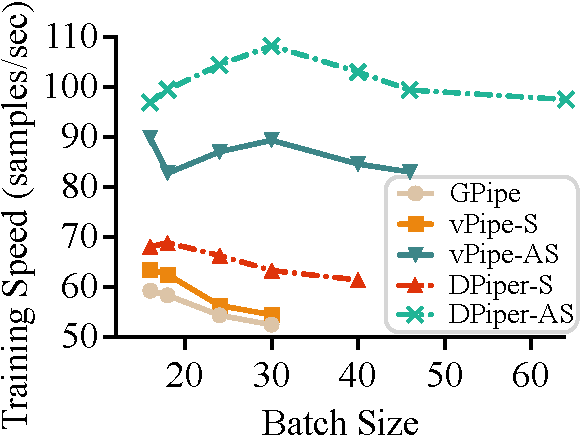
\includegraphics[width=0.47\linewidth]{BERT-4GPU-crop.pdf}
  }
  \subfigure[GPT-2]{
    \centering
    \label{subfig:gpt-2-4}
    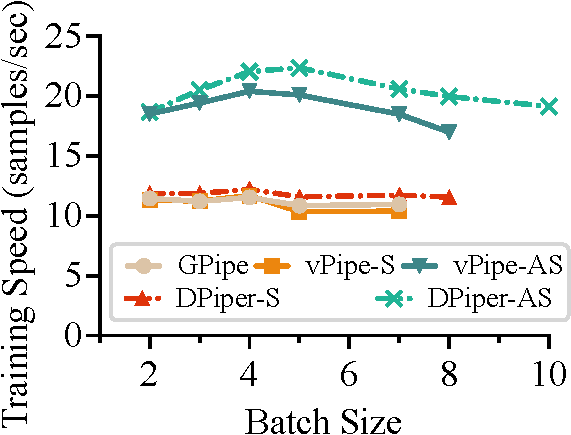
\includegraphics[width=0.47\linewidth]{GPT-2-4GPU-crop.pdf}
  }
  \subfigure[T5]{
    \centering
    \label{subfig:t5-4}
    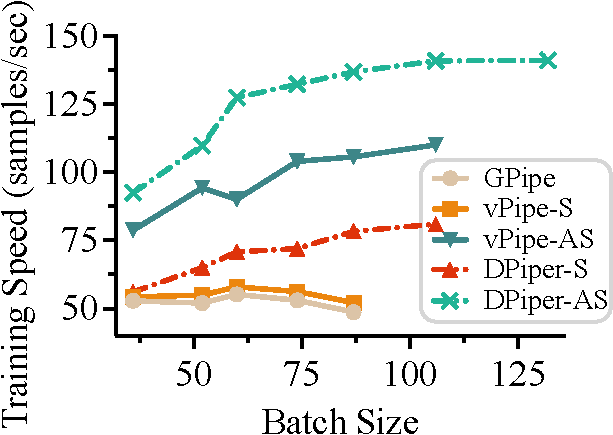
\includegraphics[width=0.47\linewidth]{T5-4GPU-crop.pdf}
  }
  \subfigure[AmoebaNet]{
    \centering
    \label{subfig:amoebanet-4}
    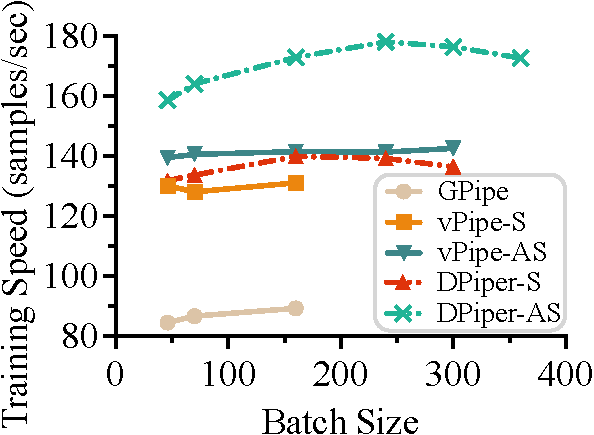
\includegraphics[width=0.47\linewidth]{AmoebaNet-4GPU-crop.pdf}
  }
  \caption{Training Speed under Pipeline Stage of 4}
  \label{fig:perf-4}
\end{figure}
% because except for a more obvious difference in the model division on AmoebaNet,
% the differences on the other three models are relatively small.

% This is because in the experiments of this chapter, the number of micro-batches executed simultaneously
% in the first stage of both synchronous and asynchronous pipeline parallelism is consistent,
% so an effective comparison can be made. 

% It should be noted that since the ZeRO and PipeDream methods
% do not perform memory optimization operations,
% they can only run at the initial batch size before memory overflow,
% so they are excluded for comparison.
% However, a brief explanation of the training performance of the ZeRO method is that as the model scale increases,
% the data parallelism will start to show a significant performance decline compared to pipeline parallelism
% due to the large amount of communication.
% For example, ZeRO's training speed on the relatively small BERT model is 1.4$\times$ that of GPipe at a smaller batch size,
% but on the larger GPT-2 model, the training speed drops to only 20\% of GPipe.
% As for PipeDream, its performance at the trainable batch size can refer to vPipe-AS,
% because except for a more obvious difference in the model division on AmoebaNet,
% the differences on the other three models are relatively small.

The training speed comparison results when pipeline stage is 4 is shown as Figure~\ref{fig:perf-4}.
% For the case of a pipeline stage number of 4,
% the training speed comparison of each method on the 4 models is shown in Figure~\ref{fig:perf-4}.
The training performance of synchronous pipeline parallelism
is significantly lower than that of the asynchronous pipeline parallelism
due to the pipeline bubbles caused by the computation synchronization.
% its training performance is significantly lower than that of asynchronous pipeline methods.
The performance of vPipe-S is generally better than GPipe,
and the advantage is more obvious on AmoebaNet,
because GPipe does not consider communication overhead between stages,
and an unreasonable partition on CNN models is more
likely to cause larger communication volumes,
while both DawnPiper and vPipe have considered the communication overhead in pipeline partition.

At a small batch size, DawnPiper does not have a particularly large advantage over other methods,
with an average performance improvement of about 7\%, and only a 17\% and 14\% performance improvement
in the asynchronous training mode on the T5 and AmoebaNet models, respectively.
Because DawnPiper can only rely on a more refined pipeline partition space
to find a better model partition when the memory is not oversubscribed.
As the batch size increases, other methods need to
perform memory optimization to meet the memory requirements for model training.
DawnPiper has a noticeable stage of increased training speed compared to other methods.
This improvement results from two folds, on the one hand,
the GPU compute resources can be better utilized when the batch size increases.
On the other hand, DawnPiper can:
a) adjust the memory footprint of each stage with minimal impact on the computation time;
b) reduce the memory footprint with almost no performance overhead by memory swapping
when the batch size is relatively small.
The first point can be achieved due to the observation on the memory usage
characteristics during training which is described in Section~\ref{sec:mot}.
% because it can make more full use of GPU resources when the batch increases from small to large,
% and on the other hand, it is also because DawnPiper can: 1) Change the memory occupation between pipeline stages
% with minimal impact on the computation of the pipeline stages;
% 2) Reduce memory occupation with almost no performance overhead by memory swapping when the batch is small.
Therefore, in synchronous pipeline parallelism,
DawnPiper achieved up to 1.5$\times$ performance improvement
on the T5 model when the batch size increased,
and up to 1.41$\times$ in the asynchronous mode.
Overall, as the batch size increases,
DawnPiper has an average performance improvement of 1.2$\times$, 1.12$\times$,
1.32$\times$, and 1.24$\times$ over vPipe in the asynchronous parallel training
on BERT, GPT-2, T5, and AmoebaNet, respectively.

The evaluations are only performed on GPT-2 and T5 as the pipeline stages increases to 8,
since the model sizes of BERT and AmoebaNet are too small for 8 GPUs.
The results are shown as Figure~\ref{fig:perf-8}.
% When the number of pipeline stages increases to 8,
% the evaluations on BERT and AmoebaNet are excluded
% since their model size is too small for 8 GPUs.
% The training speed results of GPT-2 and T5 are shown as Figure~\ref{fig:perf-8}.
% due to the size of the BERT model and the AmoebaNet model being too small relative to 8 GPUs,
% resulting in a relatively small amount of computation after division for each stage,
% this section only tests the GPT-2 model and the T5 model on 8 GPUs, which is shown as Figure~\ref{fig:perf-8}.
In the synchronous mode, the performance of GPT-2 on DawnPiper, GPipe, and vPipe is quite similar.
This is because the balanced partition positions of computation and memory for GPT-2
are very close, thus the partition optimization space is very limited.
% For the GPT-2 model, in the synchronous pipeline mode, the performance of DawnPiper, GPipe, and vPipe
% is quite close because their balanced division of computation and memory is very similar,
% thus the space for optimization is very limited.
In the asynchronous mode,
as the batch size gradually increases,
DawnPiper's training speed is by average 1.15$\times$ and 1.34$\times$
faster than vPipe on GPT-2 and T5, respectively.
DawnPiper has a better performance improvement on T5
due to its mixed model architecture based on encoder and decoder,
which has a more complex structure for providing partition space for DawnPiper.
% The T5 model, due to its being a Transformer model with a mix of encoder and decoder,
% has a more complex structure, providing more division space for DawnPiper,
% hence DawnPiper's performance improvement over vPipe is also greater.
Moreover, when the pipeline stages increase to 8,
DawnPiper also demonstrates good scalability.

\begin{figure}[htb]
  \centering
  % \hspace{-0.7cm}
  \subfigure[GPT-2]{
    \centering
    \label{subfig:gpt-2-8}
    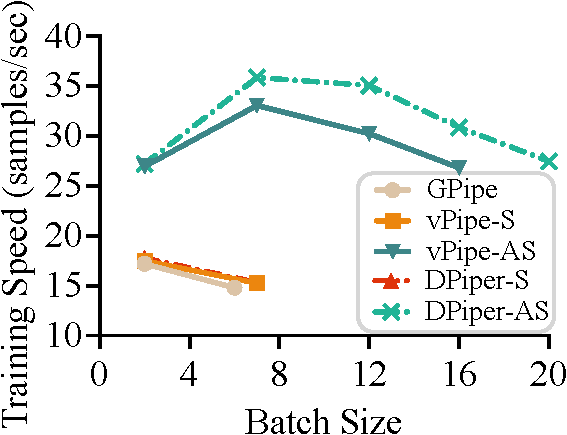
\includegraphics[width=0.47\linewidth]{GPT-2-8GPU-crop.pdf}
  }
  \subfigure[T5]{
    \centering
    \label{subfig:t5-8}
    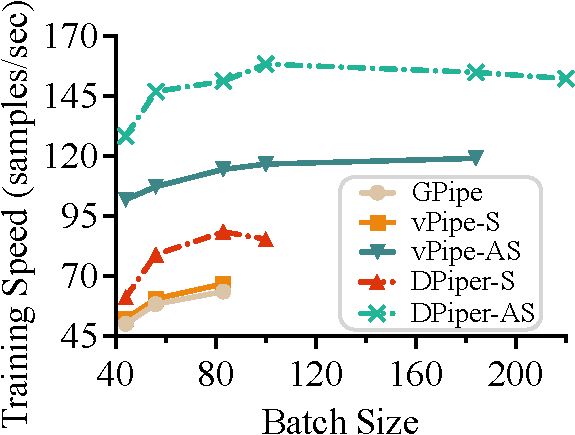
\includegraphics[width=0.47\linewidth]{T5-8GPU-crop.pdf}
  }
  \caption{Training Speed under Pipeline Stage of 8}
  \label{fig:perf-8}
\end{figure}

\subsection{Detailed analysis on computation time and memory footprint}
To provide a more detailed comparison on the memory footprint and computation of DawnPiper and vPipe,
we profile the GPU peak memory usage and computaiton time
of each stage on T5 in asynchronous mode under the pipeline stage of 8.
The micro-batch size is 110 which exceeds the maximum batch size that vPipe
can achieve without memory optimization by 2.5$\times$.
The results are shown in Figure~\ref{fig:mem-comp}. 
% this section selects the GPU memory usage and computation time
% of each stage after the division of the T5 model by vPipe and DawnPiper
% when the asynchronous pipeline stage number is 8,
% with a micro-batch size of 110, which exceeds the maximum batch size that vPipe
% can achieve without memory optimization by 2.5$\times$.
% The results are shown in Figure~\ref{fig:mem-comp}. 

Firstly, regarding to the peak memory usage of each stage,
it can be seen that DawnPiper occupies more GPU memory than vPipe
and the memory usage of each stage is more balanced.
This is because vPipe performs a coarser-grained pipeline partition and memory optimization,
while DawnPiper perform finer-grained memory optimization
to meet the memory requirements of each stage.
The overall GPU memory utilization is improved by 17.8\% compared to vPipe. 
In the meantime, the computation time of each stage under
DawnPiper's partition strategy also becomes more balanced,
with the difference between the longest and shortest execution time stages being only 7.7\%.
This ratio reaches 35.8\% under the vPipe's partition and memory optimization strategy

\begin{figure}
  \centering
  \includegraphics*[width=0.8\linewidth]{mem-comp.pdf}
  \caption{Peak Memory Usage and Computation time Analysis}
  \label{fig:mem-comp}
\end{figure}
